\chapter{Examples of Asset Bubble Detection}
\begin{enumerate}
  \item 1 example of asset bubble detection
  \begin{itemize}
    \item stock
    \item day of data
    \item table of grid points
    \item identify usable grid points.
    \item floren zmirou graph
    \item spline graphs together
    \item bubble test.
    \item Conclusion
  \end{itemize}
\end{enumerate}
% %THIS IS HOW TO PLACE FIGURES EXACTLY WHERE YOU WANT THEM
% %\begin{figure}[h]
% %\begin{center}
% %\includegraphics[scale=1]{graphics/diskPackingTheoremExample.pdf}
% %\end{center} 
% %\caption{This example represents a disk arrangement transformed to and from its corresponding graph 
% %$G_2$}
% %\label{fig:DiskArrangement-1}
% %\end{figure}
% %THIS IS HOW TO PLACE FIGURES EXACTLY WHERE YOU WANT THEM
% %FOR FURTHER REFERENCE, READ http://en.wikibooks.org/wiki/LaTeX/Floats,_Figures_and_Captions#Keeping_floats_in_their_place
% \chapter{Numerical Solution, Conclusion and Future Work}
% We will provide examples which will give better understanding toward our problem.
% {Numberical Solutions using implementation}
% \section{Examples}
% \subsection{EXAMPLE 1}
% \begin{itemize}
%   \item Ticker: \textbf{MWI Veterinary Supply Inc}
%   \item  D : 05/16/2014
%   \item  T : 60 seconds
% \end{itemize}
% \textbf{Stock Class }\\
% % \begin{figure}[h]
% % \begin{center}
% % 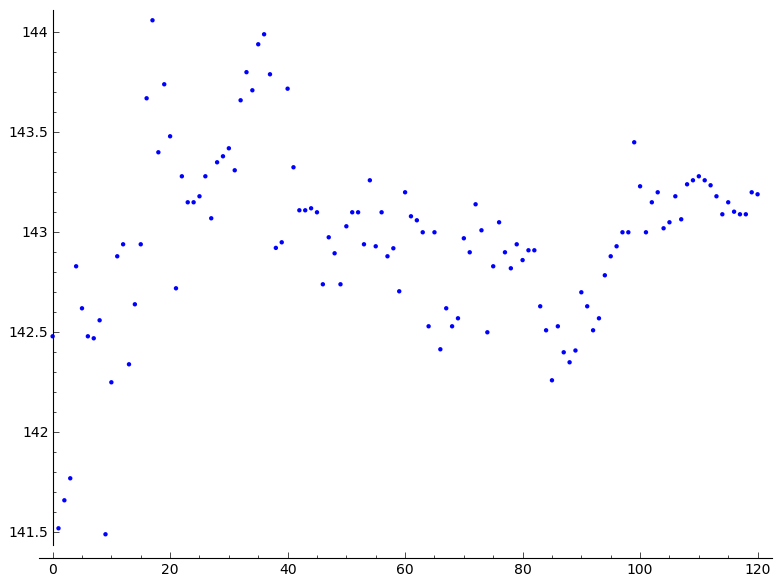
\includegraphics[scale=0.40]{MWIV_stock_price.png}
% % \end{center}
% % \caption{Stock Prices vs. Time}
% % \label{fig:Stock Price}
% % \end{figure}
% \newpage
% Now we are going to check some stocks using Stock class.Information can be downloeded from following Google Finance. We have stock prices for MWI Veterinary. The stock Price graph shows the presence of asset bubble.
% Next, Floren Zmirou estimator can be used to see the volatility of stock prices.\\\\
% \textbf{Floren Zmirou Class}
% \begin{center}
% \begin{equation}\label{florenZmirouEquation}
% S_n(x) = \frac{\Sigma_{i=1}^{n} 1_{\{|S_{t_i}-x|<h_n\}} n (S_{t_i+1}-S_{t_i})^2}{\Sigma_{i=1}^{n} 1_{\{|S_{t_i}-x|<h_n\}}}
% \end{equation}
% \end{center}
% 
% 
% \begin{tabular}{|1|c|r|}
% \hline
% Usable Grid Points  &  Estimated Sigma Zmirou  & Number of Points\\
% \hline
% 141.842890874       &           1897.69862662  &              50\\
% \hline
% 144.17445437        &          290.806107556   &            108\\
% \hline
% 143.008672622       &           464.127160557  &              60\\
% \hline
% \end{tabular}
% \\\\\\\\
% We picked $hn = \frac{1}{n^(1/3)}$. By theorem (1.17) $(h_n)_n�1 $satisfies $nh_n\rightarrow \infty $ and $nh_4n\rightarrow 0$, then $S_n(x)$ is a consistent estimator of $\sigma^2(x)$.There are Floren Zmirou's estimated sigma values for 
% usable grid points and number of points in each usable grid point. We deleted those grid points which has less than 1 percent of data.
% We are using 3 point grid.
% % \begin{figure}[h]
% % \begin{center}
% % 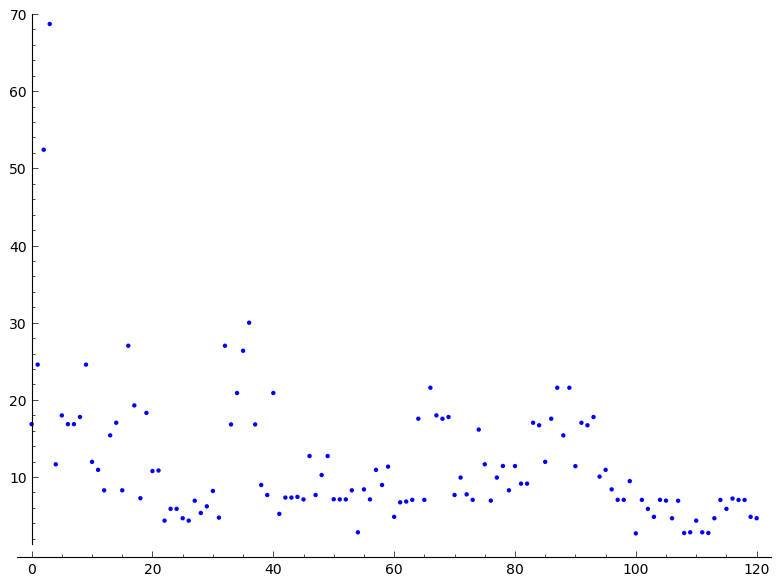
\includegraphics[scale = 0.40]{MWIV_FZ_stddev_estimation.png}
% % \end{center}
% % \caption{Stock Prices vs.Floren Zmirou Standard Deviation Estimation}
% % Next we will need to interpolate $\sigma(x)$. We used Varince of Cubic spline and Standard Deviation of cubic spline.
% % Floren Zmirou's sigma points. 
% % \label{fig:Floren Zmirou Estimation}
% % \end{figure}
% \newpage
% \textbf{Cublic Spline}
% % \begin{figure}[h]
% % \begin{center}
% % 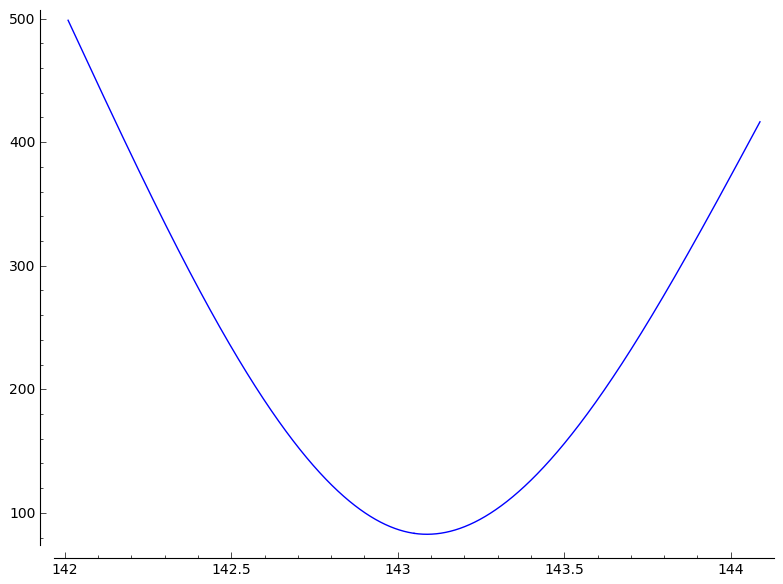
\includegraphics[scale=0.50]{MWIV_variance_spline.png}
% % \end{center}
% % \caption{Floren Zmirou Standard Deviation Estimation vs. Variance Cubic Spline}
% % \label{fig:Cubic Spline}
% % \begin{center}
% % \includegraphics[scale=0.45]{MWIV_stddev_spline.png}
% % \end{center}
% % \caption{Floren Zmirou Standard Deviation Estimation vs.Standard Deviation Cubic Spline}
% % \label{fig:Cubic Spline}
% % \end{figure}
% \\
% If the graph of the volatility versus the stock price tends to infinity at a faster rate than does the graph $f(x)=x$
% , then we have bubble.Figure 1.3 and 1.4 shows that volatility function goes to infinity at faster rate so we can conclude that
% there is a bubble in MWIV stock.The price process under a risk neutral measure is a strick local martingale.
% \\
% %%%%%%%%%%%%%%%%%%%%%%%%%%%%%%%%%%%%%%%%%%%%%%%%%%%%%%%%%%%%%%%%%%%%%%%%%%%%%%%%%%%%%%%
% \subsection{EXAMPLE 2}
% \begin{itemize}
%   \item Ticker:\textbf{ GOOGLE Inc.}
%   \item  D : 05/16/2014
%   \item  T : 60 seconds
% \end{itemize}
% \textbf{Stock Class: }\\
% \begin{figure}[h]
% \begin{center}
% \includegraphics[scale=0.40]{GOOG_stock_price.png}
% \end{center}
% \caption{Stock Prices vs. Time}
% \label{fig:Stock Prices}
% \end{figure}
% \\
% Figure 1.5 is showing stock prices for Google Inc. We do not see the existence of an asset bubble. Since the prices are going upward, it is hard to conclude.
% We will see how the volatility will look for these stock prices.\\\\
% \newpage
% \textbf{Floren Zmirou Class}
% \\
% \begin{tabular}{|1|c|r|}
% \hline
% Usable Grid Points &   Estimated Sigma Zmirou  & Number of Points\\
% \hline
% 547.289611925      &            267.623605573  &              64\\
% \hline
% 549.612686541      &            517.868135963  &             143\\
% \hline
% 551.935761158      &           76.0733825073   &              17\\
% \hline
% 544.966537308      &               1890.46832  &               72\\
% \hline
% \end{tabular}
% \begin{figure}[h]
% \begin{center}
% \includegraphics[scale=0.50]{GOOG_FZ_stddev_estimation.png}
% \end{center}
% \caption{Floren Zmirou Standard Deviation Estimation vs. Stock Prices}
% \label{fig:Floren Zmirou}
% \end{figure}
% We are using 4 points grid in this example. As we see in figure 1.6, the sigma values are widely distributed so it is very difficult to conclude
% from $\sigma(x)$ values. We will interpolate by cubic spline to see the behaviour of volatility function.\\
% \newpage
% \textbf{Cublic Spline}
% \begin{figure}[h]
% \begin{center}
% \includegraphics[scale=0.50]{GOOG_variance_spline.png}
% \end{center}
% \caption{Floren Zmirou Standard Deviation Estimation vs. Variance Cubic Spline}
% \label{fig:Cubic Spline}
% \begin{center}
% \includegraphics[scale=0.45]{GOOG_stddev_spline.png}
% \end{center}
% \caption{Floren Zmirou Standard Deviation Estimation vs.Standard Deviation Cubic Spline}
% \label{fig:Cubic Spline}
% \end{figure}
% \\
% Figure 1.7 and 1.8 shows that the $\sigma(x)$ values goes to 0. The graphs are not going to infinity, so
% we can conclude that there is no bubble in asset prices. Therefore it is martingale.
% \newpage
% %%%%%%%%%%%%%%%%%%%%%%%%%%%%%%%%%%%%%%%%%%%%%%%%%%%%%%%%%%%%%%%%%%%%%%%%%%%%%%%%%%%%%%%
% \subsection{EXAMPLE 3}
% \begin{itemize}
%   \item Ticker: \textbf{APPLE Inc.}
%   \item  D : 05/21/2014
%   \item  T : 60 seconds
% \end{itemize}
% \textbf{Stock Class}
% \begin{figure}[h]
% \begin{center}
% 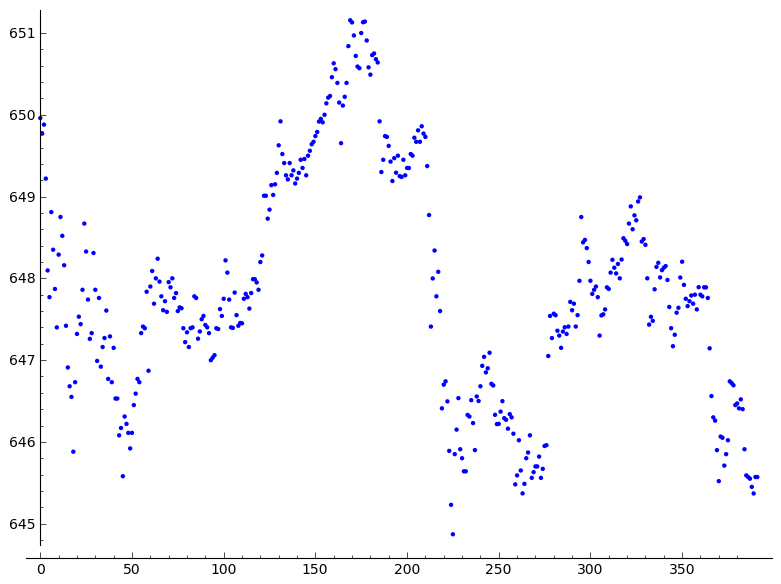
\includegraphics[scale=0.40]{AAPL_stock_price.png}
% \end{center}
% \caption{Stock Prices vs. Time}
% \label{fig:Stock Price}
% \end{figure}
% \\
% Here we have stock prices for Apple for one day in seconds. We tested the existence of bubble. Results are inconclusive but we still can not see bubble in price.
% We will have better understanding about volatility function in Floren Zmirou's estimation graph.\\\\
% \textbf{Floren Zmirou Estimation}\\
% \begin{center}
% \begin{equation}\label{florenZmirouEquation}
% S_n(x) = \frac{\Sigma_{i=1}^{n} 1_{\{|S_{t_i}-x|<h_n\}} n (S_{t_i+1}-S_{t_i})^2}{\Sigma_{i=1}^{n} 1_{\{|S_{t_i}-x|<h_n\}}}
% \end{equation}
% \end{center}
% \\
% \begin{tabular}{|1|c|r|}
% \hline
% Usable Grid Points &   Estimated Sigma Zmirou &  Number of Points\\
% \hline
% 602.871457276      &           138.351149247      &           42\\
% \hline
% 603.874371827      &            245.251175157     &           125\\
% \hline
% 604.877286378      &            102.97102087      &          104\\
% \hline
% \end{tabular}
% \begin{figure}[h]
% \begin{center}
% 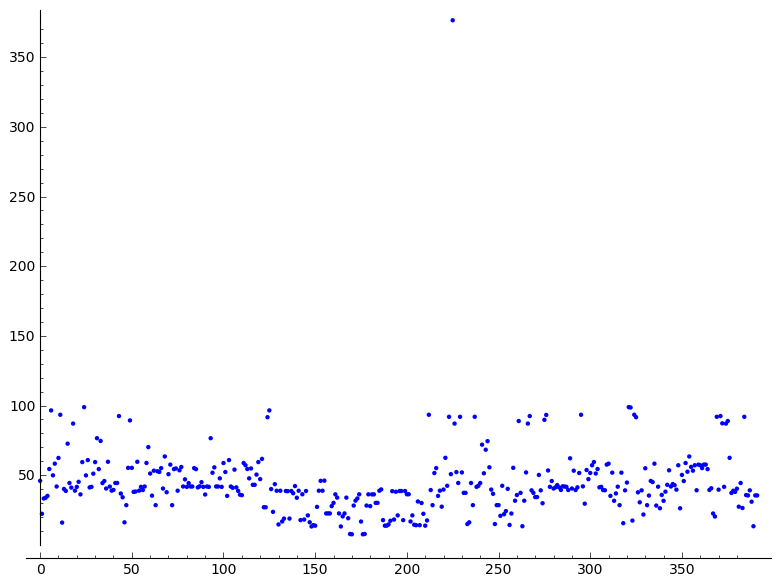
\includegraphics[scale=0.50]{AAPL_FZ_stddev_estimation.png}
% \end{center}
% \caption{Floren Zmirou Standard Deviation Estimation vs. Stock Prices}
% \label{fig:Floren Zmirou Estimation}
% \end{figure}
% \\\\
% \newpage
% We are using 3 points grid. We can not conclude if the volatility funcion $\sigma(x)$ is going to infinity or not in figure 1.10.
% We will interpolate $\sigma(x)$ to see the behaviour of the volatility function.
% \newpage
% \textbf{Cublic Spline}
% \begin{figure}[h]
% \begin{center}
% 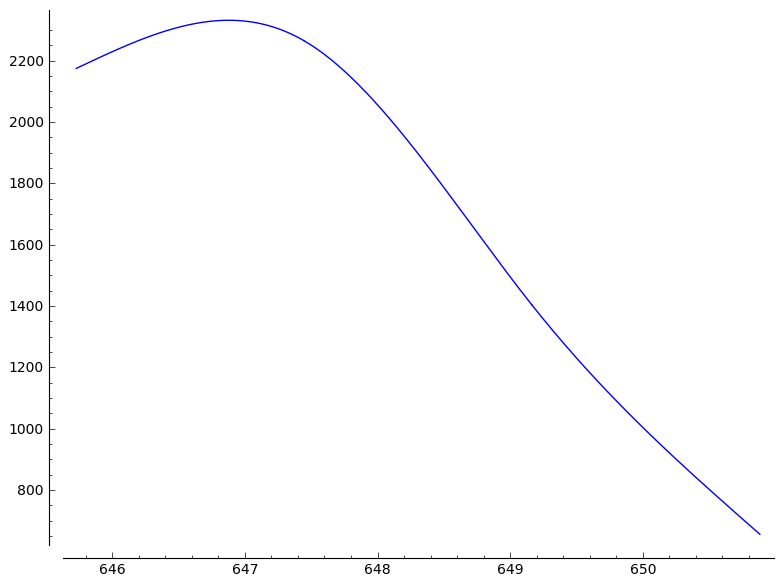
\includegraphics[scale=0.50]{AAPL_variance_spline.png}
% \end{center}
% \caption{Floren Zmirou Standard Deviation Estimation vs. Variance Cubic Spline}
% \label{fig:Cubic Spline}
% \begin{center}
% \includegraphics[scale=0.45]{AAPL_stddev_spline.png}
% \end{center}
% \caption{Floren Zmirou Standard Deviation Estimation vs.Standard Deviation Cubic Spline}
% \label{fig:Cubic Spline}
% \end{figure}
% \\
% Figure 1.11 and 1.12 shows that the $\sigma(x)$ goes to 0 as $x$ goes to infinity so under the risk neutral probabilities, Apple asset price is a martingale therefore
% there is no bubble in the price.
% 
% %%%%%%%%%%%%%%%%%%%%%%%%%%%%%%%%%%%%%%%%%%%%%%%%%%%%%%%%%%%%%%%%%%%%%%%%%%%%%%%%%%%%%%%
% \newpage
% \subsection{EXAMPLE 4}
% \begin{itemize}
%   \item Ticker: \textbf{GROUPON Inc.}
%   \item  D : 05/21/2014
%   \item  T : 60 seconds
% \end{itemize}
% \textbf{Stock Class}
% \begin{figure}[h]
% \begin{center}
% 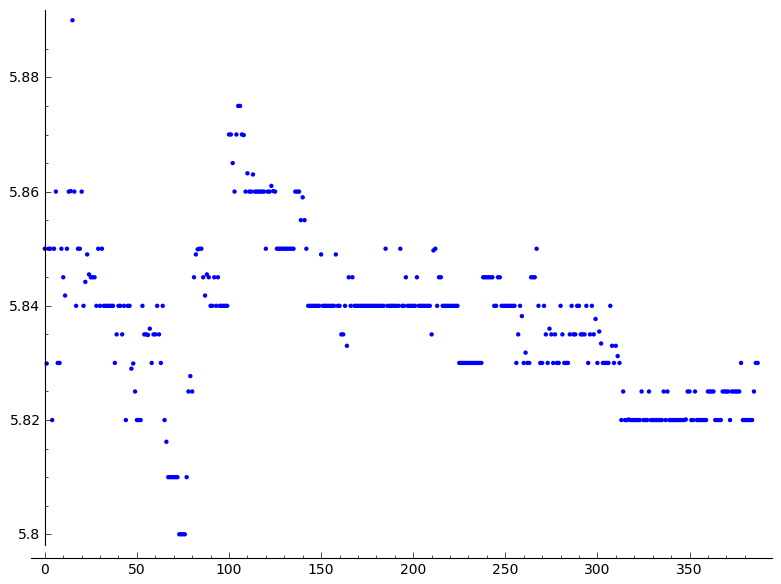
\includegraphics[scale=0.40]{GRPN_stock_price.png}
% \end{center}
% \caption{Stock Prices vs. Time}
% \label{fig:Stock Price}
% \end{figure}
% \\
% Figure 1.13 shows that stock prices of Groupon are going to infinity as time increases. We can not determine determine the exsitence of bubble.\\\\
% \textbf{Floren Zmirou Estimation}\\
% \begin{center}
% \begin{equation}\label{florenZmirouEquation}
% S_n(x) = \frac{\Sigma_{i=1}^{n} 1_{\{|S_{t_i}-x|<h_n\}} n (S_{t_i+1}-S_{t_i})^2}{\Sigma_{i=1}^{n} 1_{\{|S_{t_i}-x|<h_n\}}}
% \end{equation}
% \end{center}
% 
% \begin{tabular}{|1|c|r|}
% \hline
% Usable Grid Points  &  Estimated Sigma Zmirou &  Number of Points\\
% \hline
% 6.01159662403       &        0.0106001479673  &             25\\
% \hline
% 6.0947898721        &        0.00331796023881 &              38\\
% \hline
% 6.17798312017       &       0.000229293586847 &              155\\
% \hline
% 6.26117636824       &      7.51642424675e-05  &              86\\
% \hline
% \end{tabular}
% \begin{figure}[h]
% \begin{center}
% 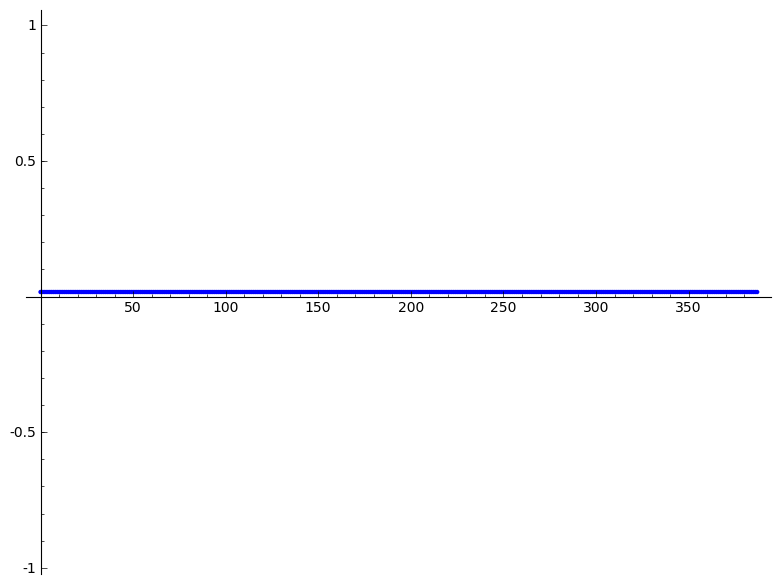
\includegraphics[scale=0.50]{GRPN_FZ_stddev_estimation.png}
% \end{center}
% \caption{Floren Zmirou Standard Deviation Estimation vs. Stock Prices}
% \label{fig:Stock Price}
% \end{figure}
% \\
% \newpage
% There are 4 points grid which we are using in this example. Floren Zmirou Estimated Sigma values are very small.
% In Figure 1.14, $\sigma(x)$ values are going to $\infty$ as $x$ goes to $\infty$. We will interpolate for better results.
% \newpage
% \textbf{Cublic Spline}
% \begin{figure}[h]
% \begin{center}
% 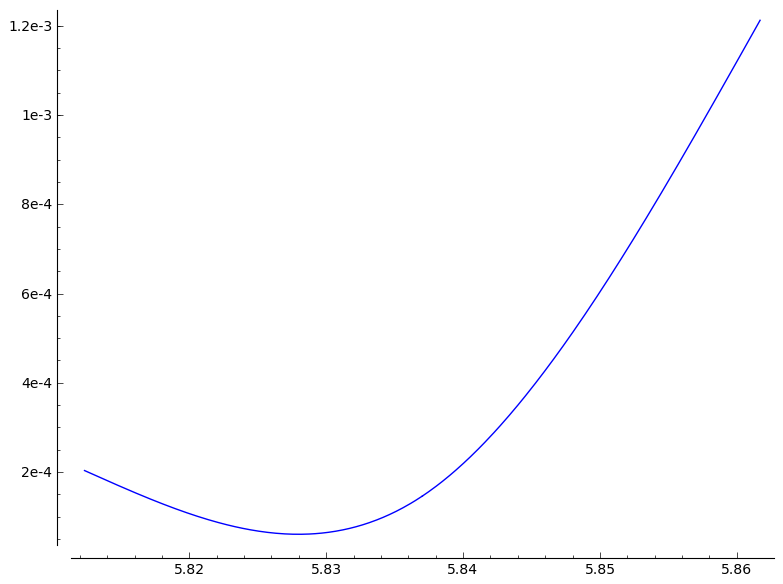
\includegraphics[scale=0.40]{GRPN_variance_spline.png}
% \end{center}
% \caption{Floren Zmirou Standard Deviation Estimation vs. Variance Cubic Spline}
% \label{fig:Cubic Spline}
% \begin{center}
% \includegraphics[scale=0.40]{GRPN_stddev_spline.png}
% \end{center}
% \caption{Floren Zmirou Standard Deviation Estimation vs.Standard Deviation Cubic Spline}
% \label{fig:Cubic Spline}
% \end{figure}
% \\
% Figure 1.15 and 1.16 shows that volatility function is going to infinity as $x$ values are going to infinity so groupon asset price is a supermartingale
% therefore we can conclude that there is a bubble in asset price.
% \newpage
% \section{Future Work}
% \begin{itemize}
%   \item Still need to know tail of the volatility function.
%   \item Need to extrapolate the volatility with either Comparison Theorem Method or Reproducing Kernal Hilbert Spaces.
%   \item Need to know themorem 0.1.12 equation(3)
%   \begin{equation}
%   \int_\alpha^\infty \frac{x}{\sigma^2(x)}dx < \infty
%    \end{equation} 
%    for all $\alpha > 0$ is finite or infinite.
%   \item Determine from intergral if there is bubble or not.
% \end{itemize}
